% !TEX root = main.tex

\chapter{Pictures}
\usepackage{tikz}

%------------------------------
\section*{The \LaTeX\ \texttt{picture} environment}

\autoref{fig:heron} was created with the \LaTeX\ {\tt picture} environment.

\begin{figure}[htb]
\centering
\setlength{\unitlength}{0.8cm}
\begin{picture}(6,5)
\thicklines
\put(1,0.5){\line(2,1){3}}
\put(4,2){\line(-2,1){2}}
\put(2,3){\line(-2,-5){1}}
\put(3.1,2.5){$a$}
\put(1.2,1.7){$b$}
\put(2.5,0.95){$c$}
\put(0.3,4){$\text{Area}=\sqrt{s(s-a)(s-b)(s-c)}$}
\put(3.5,0.4){$\displaystyle s:=\frac{a+b+c}{2}$}
\end{picture}
\caption{Heron's formula.\label{fig:heron}}
\end{figure}

%------------------------------
\section*{Tikz pictures}

\autoref{fig:koch} was created with {\tt tikz}.

\begin{figure}[htb]
\centering
\usetikzlibrary{decorations.fractals}
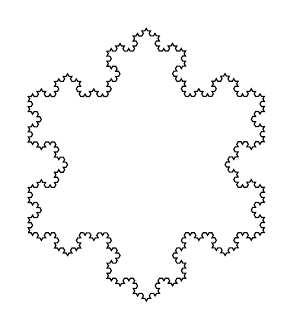
\begin{tikzpicture}[decoration=Koch snowflake]
   \draw decorate{ decorate{ decorate{ decorate{
        (0,0) -- ++(60:3)  -- ++(300:3) -- ++(180:3)}}}};
\end{tikzpicture}
\caption{Koch snowflake.\label{fig:koch}}
\end{figure}

%------------------------------
%\section*{Camel System Architecture}
\usetikzlibrary{shapes.geometric, arrows}
\makeatletter
\pgfarrowsdeclare{crow's foot}{crow's foot}
{
  \pgfarrowsleftextend{+-.5\pgflinewidth}%
  \pgfarrowsrightextend{+.5\pgflinewidth}%
}
{
  \pgfutil@tempdima=1.2pt%
  \advance\pgfutil@tempdima by.25\pgflinewidth%
  \pgfsetdash{}{+0pt}%
  \pgfsetmiterjoin%
  \pgfpathmoveto{\pgfqpoint{0pt}{-6\pgfutil@tempdima}}%
  \pgfpathlineto{\pgfqpoint{-6\pgfutil@tempdima}{0pt}}%
  \pgfpathlineto{\pgfqpoint{0pt}{6\pgfutil@tempdima}}%
  \pgfusepathqstroke%
}
\makeatother
\tikzstyle{nobox} = [minimum width=10ex, minimum height=4ex,text centered, draw=none]
\tikzstyle{basic} = [rectangle, rounded corners, minimum width=12ex, minimum height=5ex,text centered, draw=black]
\tikzstyle{django} = [rectangle, rounded corners, minimum width=12ex, minimum height=5ex, text centered, draw=black, fill=green!30]
\tikzstyle{arrow} = [ultra thick,->,>=latex]

\begin{figure}[htb]
\centering
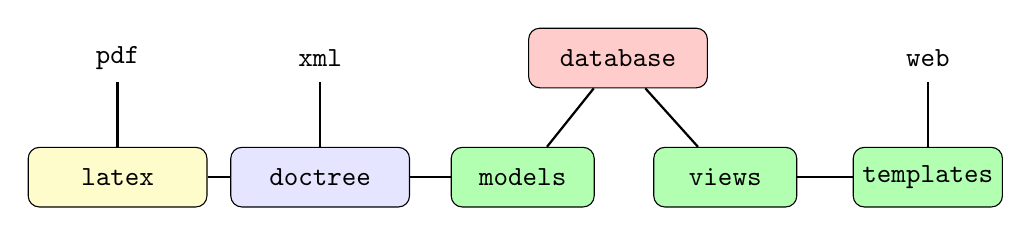
\begin{tikzpicture}[font=\ttfamily, node distance=10ex]
\node (pdf) [nobox] {pdf};
\node (xml) [nobox, right of=pdf, xshift=7ex] {xml};
\node (latex) [basic, fill=yellow!20, below of=pdf] {\texttt{latex}};
\node (doctree) [basic, fill=blue!10, right of=latex, xshift=7ex] {doctree};
\node (models) [django, right of=doctree, xshift=7ex] {models};
\node (database) [basic, fill=red!20, right of=xml, xshift=15ex] {database};
\node (views) [django, right of=models, xshift=7ex] {views};
\node (templates) [django, right of=views, xshift=7ex] {templates};
\node (web) [nobox, right of=database, xshift=16ex] {web};
\draw [arrow] (latex) -- (doctree);
\draw [arrow] (latex) -- (pdf);
\draw [arrow] (doctree) -- (xml);
\draw [arrow] (doctree) -- (models);
\draw [arrow] (models) -- (database);
\draw [arrow] (database) -- (views);
\draw [arrow] (views) -- (templates);
\draw [arrow] (templates) -- (web);
\end{tikzpicture}
\caption{System architecture.\label{fig:architecture}}
\end{figure}

%------------------------------
%\section*{Database schema}

\tikzstyle{basic} = [rectangle, rounded corners, minimum width=15ex, minimum height=5ex,text centered, draw=black]
\tikzstyle{arrow} = [thick,-,>=latex]
\begin{figure}[htb]
\begin{center}
\begin{tikzpicture}[font=\ttfamily, node distance=10ex]
\node (student) [basic, fill=green!10] {student};
\node (module) [basic, fill=red!10, right of=student, xshift=15ex] {module};
\node (book) [basic, fill=blue!10, right of=module, xshift=15ex] {book};
\node (submission) [basic, fill=green!10, below of=student, yshift=-5ex] {submission};
\node (homework) [basic, fill=blue!10, below of=module, yshift=-5ex] {homework};
\node (answer) [basic, fill=green!10, below of=submission, yshift=-5ex] {answer};
\node (question) [basic, fill=blue!10, below of=homework, yshift=-5ex] {question};
\draw [arrow] [thick, crow's foot-crow's foot] (student) -- (module);
\draw [arrow] [-crow's foot] (module) -- (book);
\draw [arrow] [-crow's foot] (student) -- (submission);
\draw [arrow] [-crow's foot] (submission) -- (answer);
\draw [arrow] [-] (submission) -- (homework);
\draw [arrow] [-crow's foot] (module) -- (homework);
\draw [arrow] [-crow's foot] (homework) -- (question);
\draw [arrow] [-crow's foot] (question) -- (answer);
\end{tikzpicture}
\end{center}
\caption{Database schema.\label{fig:schema}}
\end{figure}
